\documentclass[12pt, openany]{book}
\usepackage{amsmath}
\usepackage{amsthm}
\usepackage{amstext}
\usepackage{amsopn}
\usepackage[round]{natbib}
\usepackage{subfigure}
\usepackage{graphicx}



\usepackage{texdraw}    %texdraw package
\usepackage{float}
\usepackage{url}

\textwidth 160mm \textheight 210mm \oddsidemargin 15pt
\evensidemargin 0pt \topmargin 0cm \headsep 0.3cm
\renewcommand\baselinestretch{1.5}

\newtheorem{theorem}{Theorem}[chapter]
\newtheorem{lemma}[theorem]{Lemma}
\newtheorem{proposition}[theorem]{Proposition}
\newtheorem{corollary}[theorem]{Corollary}

\theoremstyle{definition}
\newtheorem{definition}[theorem]{Definition}
\newtheorem{example}[theorem]{Example}
\newtheorem{xca}[theorem]{Exercise}

\theoremstyle{remark}
\newtheorem{remark}[theorem]{Remark}

\numberwithin{equation}{chapter}
\numberwithin{figure}{chapter}

\begin{document}

\frontmatter
\title{Species Invasion in a Network Population Model}
\author{{\large Ryan C. Yan} \\
\\
{\small Department of Applied Science,}\\
{\small College of William and Mary,}\\
{\small Williamsburg, VA 23187-8795, USA }\\
\\
{\small Email:  rcyan@email.wm.edu }}
\date{}
\maketitle


\pagestyle{plain}

\newcommand{\ds}{\displaystyle}
\newcommand{\ep}{\varepsilon}
\newcommand{\la}{\lambda}
\newcommand{\R}{{\mathbf R}}
\newcommand{\Rp}{{\mathbf R}^+}
\newcommand{\rn}{{\mathbf R}^n}
\newcommand{\noi}{\noindent}


\maketitle

\begin{center}
\begin{minipage}{120mm}
\begin{center}{\bf Abstract}\end{center}

The introduction and spread of invasive species is increasingly driven by the expansion of human-made transportation routes. We formulate a network model of biotic invasion incorporating logistic growth and dispersal along a network, and present analyses of the model. We introduce small world networks and use them to investigate the role of network properties and long-distance dispersal on spread dynamics. Lastly we present comparisons between the stochastic and deterministic models to illustrate the effects of stochasticity on invasive species spread dynamics.

\end{minipage}
\end{center}
\setcounter{page}{2}

\tableofcontents

{\listoffigures \let\cleardoublepage\clearpage}
 \mainmatter

\chapter{Introduction}

\section{Background on Invasive Species}

The National Invasive Species Council defines invasive species as non-native species whose introduction is likely to cause harm \citep{invasive2006invasive}. As a common and pervasive cause of environmental and economic damage, the problem of invasive species has come to be one of the most pressing issues in ecology today. Invasive agricultural pests alone are estimated to cost the United States \$120 billion annually. In addition, 42\% of endangered or threatened species in the U.S. are at risk primarily due to invasive species \citep{pimentel2005update}. The severity of the problem is clear, yet attempts at guarding ourselves against invasive species introductions have historically failed, and still do. Though a portion of these failures can be contributed to sociological issues, such as lack of public awareness and government support to address the issue, we still have only a limited understanding of the spread and proliferation of terrestrial invasive species \citep{mack2000biotic}. It is the role of modelers to understand these processes well enough to produce accurate insights on them. 

The invasion process proceeds in several stages, as explained in \cite{williamson1989mathematical}. First is the introduction of propagules or organisms into the new environment. Although an introduction may occur, a large proportion of these introductions fail to establish stable colonies. Those that succeed in the establishment phase often exhibit a lag time - a period of low growth followed by rapid proliferation until the population reaches its carrying capacity \citep{mack2000biotic}. This particular pattern of accelerating and decelerating growth is called logistic growth and will be described further.
	
Once established in a central location, further range expansion can rapidly occur - the ``spread'' phase. Many different models are used to describe the spread or dispersal phase of species invasion. Historically, logistic population growth has been paired with diffusive spread to generate predictive models of species spread. Yet many species are known to be spread via long-distance dispersal events via human transport vectors \citep{carlton2003invasive}. 

Humans and animals have long acted as vectors of dispersal for invasive organisms. Gypsy moths lay their eggsacs on the underside of car bumpers, bivalves can be taken in with ballast water on ships, and exotic pest species can be shipped in infected shipments of agricultural or construction materials \citep{carlton2003invasive}. Biotic invasions have occurred long before our time (oftentimes, plant seeds are physically dispersed by hitching onto an animal or person), but since the Industrial Revolution, the rapid expansion of production alongside the development of new global trade routes has hastened the rate of introductions significantly \citep{hulme2009trade}.

The perceived importance of long-distance dispersal events in invasive species spread, particularly relating to the human-made transportation network, leads us to choose a network model framework for our research.

\section{Modeling Background}

The invasive species literature is rich with a large volume of research to draw upon to formulate our model. The purpose of this section is twofold in both motivating this study and providing a brief summary of the common modeling techniques in the invasive species literature. Throughout this thesis, we will use the terms ``node'' and ``patch'' interchangeably. Generally, a node in our network model is meant to represent a discrete population, or ``patch'' in the context of biology.

We begin by discussing models of single-patch population growth, discounting dispersal between locations for now. The most common model of population growth in biology is the continuous logistic equation, defined as:
\begin{equation}\label{logisticode}
\frac{dN}{dt} = rN\left(1 - \frac{N}{K}\right),
\end{equation}
where $N$ is the population size, $r$ is the intrinsic growth rate of the population, and $K$ is the carrying capacity.

One criticism of this model is that lacks the inclusion of an Allee effect, characterized as a positive association between population density and individual fitness. As explained in \cite{korolev2014turning}, a strong Allee effect is a phenomenon that leads a population to extinction once it dips below a certain threshold. Thus the extension of the logistic growth function with a strong Allee effect describes a population which grows at intermediate population levels but whose growth rate declines at both low and high population, becoming negative at low populations below the threshold. Allee effects can be caused by many different mechanisms that are positively density dependent, such as pack hunting behavior or mate-finding. The logistic equation can be modified to include an Allee effect as follows:
\begin{equation}\label{alleeode}
\frac{dN}{dt} = rN\left(1 - \frac{N}{K}\right)\left(\frac{N}{A} - 1\right),
\end{equation}
where $A$ is a positive constant that defines the threshold below which extinction is ensured. 

Steady states and stability for Equations \ref{logisticode} and \ref{alleeode} are shown in Figure \ref{combinedflows}. In the population undergoing logistic growth without an Allee effect (Figure \ref{combinedflows}a), the extinct state (zero population) is unstable and grows towards carrying capacity with a small positive perturbation. However, under a strong Allee effect (Figure \ref{combinedflows}b), another steady state at the Allee threshold $A$ is introduced. The extinct state becomes stable, with $A$ being unstable and the carrying capacity remaining a stable point. As discussed in Section 1.1, the introduction of a small number of individuals of an invasive species to a new location will often fail to establish a stable colony. The steady state properties of the logistic equation predict that all introductions will establish stable colonies. We know that in nature, this is not true. A likely reason for this is that many species experience population growth with positive density dependence at low populations as modeled by the logistic equation with a strong Allee effect.

\begin{figure}[t!]
\begin{center}
       
\includegraphics[width=1.0\textwidth]{combinedflows.png}
       \caption{\textbf{(a)} Flow diagram showing steady states and stability of Equation \ref{logisticode}. \textbf{(b)} Flow diagram showing steady states and stability of Equation \ref{alleeode}. \label{combinedflows}}
\end{center}
\end{figure}

The previous models describing single-patch population growth are not spatially explicit. Models of species spread combine population growth with some sort of dispersal mechanism. Historically, a common and relatively simple approach to model spatial dispersal is based on reaction-diffusion equations. An early example of this is a form of Fisher's equation, taken from \cite{neubert2004projecting}:
\begin{equation}\label{fisher}
\frac{\partial{N}}{\partial{t}} = rN\left(1-\frac{N}{K}\right) + D\frac{\partial^2{N}}{\partial{x^2}}.
\end{equation}
Here, we present a simple one-dimensional form, with $N(x,t)$ representing the population density at time $t$ and location $x$. The parameters $r$ and $K$ denote the intrinsic growth rate and the environmental carrying capacity, respectively. Finally, $D$ denotes the diffusion coefficient. This type of model presents an oversimplified view of population spread, failing to take into account variables such as age-structure or environmental factors such as landscape heterogeneity. Models with simple diffusion describe species invasion as a solid advancing front, where in reality, the spread dynamics are much more complex. For example, in recorded terrestrial invasions such as the coypu rodent in Europe and North America, the spread of the species is not synchronous, but rather there exist isolated colonies ahead of the front as well as locations behind that front that remain uncolonized by the species \citep{reeves1989application}.

Several different approaches were developed to incorporate various aspects left out by the relatively basic reaction-diffusion equations. Integro-difference equations (IDEs), as described in \cite{neubert2004projecting}, express the process of spread in two phases. For a model of population spread along a single dimension, we would first calculate the change in local population density according to the equation
\begin{equation}\label{ide1}
N(y, t+1) = f[N(y,t)],
\end{equation}
where $N(y, t+1)$ is the population density at location $y$ at time $t+1$, which is arrived at from applying a growth function $f$ on the population at time $t$. Secondly, the population is redistributed by the density kernel $k(x,y)$, the probability of redistributing from point $y$ to point $x$. The resulting distribution of population at time $t+1$ is then described by the IDE:
\begin{equation}\label{ide2}
N(x, t+1) = \int^{+\infty}_{-\infty} k(x,y)f[N(y,t)]dy.
\end{equation}
The main advantage of IDEs are their flexibility in choosing the density kernel, which allows for more complex redistribution of population. A similar type of model, integrodifferential equations, are used in \cite{sharov1998model} to model the spread of Gypsy moths in the United States. Integrodifferential models share a similar form to integrodifference models, with the difference being that the former represents continuous time processes whereas the latter is a discrete time model.

In recent years the growth in computational power and abundance and communication of ecological data has spurred the use of more data-driven species distribution models (SDMs). These models, as explained in \cite{vaclavik2009invasive}, use presence and absence data with environmental data to create a mathematical model of species distribution in environmental space. With the appropriate geographically mapped data, for example, data layers in a Geographical Information System (GIS) data set, one could generate potential landscapes that the species could inhabit. As reviewed in \cite{elith2009species}, there is much debate about model selection and predictive capabilities of SDMs. Historically SDMs have been used to explain present species distributions. However, in the case of invasive species we wish to use the model for extrapolation. One problem with SDMs is that an underlying assumption is that the species in question is in equilibrium with its environment. Essentially, this means that we expect the species to be present in all of its suitable habitats. This assumption is likely false for invasive species, since they face clear dispersal limitations being newly introduced to their environment. Despite these concerns, SDMs are increasingly being used more for extrapolations by linking them with dispersal models to generate predictions of invasive species spread.

Lastly, we reach a relatively new approach and the topic of this thesis: network models of invasive species. Networks are widely studied and applied to a multitude of fields, including invasive species biology. In this field, marine species have received more attention than terrestrial species. A recent, highly cited paper by \cite{kaluza2010complex} posed a network framework of marine bioinvasion, with links between ports weighted by observable shipping traffic along these routes. \cite{floerl2009importance} investigated transport hubs as centers for species dispersal. Using data from marinas near New Zealand, they found that locations categorized as high traffic and connectivity ``hubs'' were much more likely to be infected early and be the source of spread to many secondary locations than less visited locations. 

There have also been recent papers focused on building predictive models of terrestrial invasive species. For example, in \cite{ferrari2014modeling}, researchers presented a predictive model of hemlock woolly adelgid spread, using a dynamic network model to explore which nodes were most active in dispersal. In \cite{koch2014using}, researchers investigated the spread of forest pests in the United States and Canada via firewood movement, commonly held as a vector for forest pest introduction. Despite the acknowledged importance of these studies, much of the presently available research has been focused on case studies of particular species and their specific distribution networks. Less work has been done on the general analysis of network models of invasive species, although we are seeing a rise in their usage. 

The spread of invasive species across disparate terrestrial landscapes lends itself to modeling in a network framework. In addition, the new availability of both ecological species data and human-centric transportation data will facilitate studies such as these for terrestrial species. The goal of our research is to present a general network model of terrestrial invasive species spread and analyze the individual components of that model. This model is derived from research the author previously conducted to produce a Markov chain model of invasive species spread using commodity flow pathway data \citep{yan2015transport}. Over time, data driven, computationally-intensive models may become more attractive due to increases in data availability and computational power. This will lead us to more powerful predictive tools, but we should aim to understand the general properties of network science and invasion biology that underlie their use.

\subsection{Thesis Outline}

In this thesis we will formulate and analyze a network model of biotic invasion using steady state analysis as well as numerical modeling. We divide the thesis into three main sections in addition to the introduction and conclusion. In Chapter 2 we will derive the deterministic model and analyze its steady state properties in $1$ and $2$ dimensions. We also define the $n$ dimensional model we use for computational simulations. In Chapter 3, we introduce the characteristics of a particular type of network, small world networks, and their relation to biotic invasion. Lastly, in Chapter 4, we introduce a stochastic model and explore the role of stochasticity in different parameter regimes in the network invasion model.

\chapter{Deterministic Modeling}
\section{1-Dimensional Model Formulation}

\subsection{Rationale}
We begin by defining a single-patch model, where the dynamics are described simply by population growth. In the wider model of invasive species, this single-patch model represents the establishment phase of an invasive species in a single location. In this section, we define the time-$t$ map, the discrete time analog to the continuous logistic equation defined by Equation \ref{logisticode}. The main reason we chose not to use the continuous time logistic equation was because using our map formulation here reduced the computational time significantly over integration of the continuous logistic growth function.

\subsection{Model Specification}

We begin by deriving the discrete map analog to the standard logistic equation presented above in Equation \ref{logisticode}. This will map a population within a single patch forward in yearly time steps.

Through separation of variables and direct integration, we come to the general solution to the continuous time logistic equation:
\begin{equation}\label{generalsolution}
N(t) = \frac{Ce^{rt}}{1 + \frac{Ce^{rt}}{K}},
\end{equation}
where $C$ is the constant of integration. Setting the initial population at time zero equal to some value $N_0$, we solve for $C$, and arrive at the equation below:
\begin{equation}\label{constantofintegration}
C = \frac{N_0}{1-\frac{N_0}{K}}.
\end{equation}
Replacing $C$ in Equation \ref{constantofintegration} yields the particular solution
\begin{equation}\label{particularsolution}
N(t) = \frac{N_{0}e^{rt}}{1 + \frac{N_{0}(e^{rt}-1)}{K}}.
\end{equation}
Given an initial population value $N_0$ at time $t = 0$, we can calculate the population at $t = 1$. We define the resulting discrete map with a 1-year time step with the equation:
\begin{equation}\label{logisticmap}
N_{t+1} = g(N_t) = \frac{N_{t}e^{r}}{1 + \frac{N_{t}(e^{r}-1)}{K}}.
\end{equation}
\subsection{Alternative Logistic Models}

	A common discretization of the logistic differential equation $(1.1)$ is the standard form of the recurrence relation form shown below:
\begin{equation}\label{altlog}
N_{t+1} = rN_t\left(1 - \frac{N_t}{K}\right).
\end{equation}
Although relatively simple looking, this formulation of the discrete logistic map reveals undesirable bifurcation properties and chaos as we increase the intrinsic growth rate $r$ from $0$ to $4$.	
	We chose to use the formulation in Equation \ref{logisticmap} because of the lack of chaotic behavior at large values of $r$. Our formulation exhibits the typical sigmoidal curve characteristic of the logistic equation without atypical behavior.

\section{1-Dimensional Stability Analysis}

\subsection{Fixed points}
What are the steady state properties of the model discrete logistic map we defined in Equation \ref{logisticmap}? We discussed the steady state of the ordinary differential equation form of the logistic equation, Equation \ref{logisticode}, in Chapter 1. We expect the stability results here to reflect those of the logistic ordinary differential equation (ODE) since we derived the map from the logistic equation. We follow the approach described in \cite{strogatz1994nonlinear} to analyze the steady state stability of our discrete map system from Equation \ref{logisticmap}. We first look to discover the fixed points of the system. A fixed point of $g$ is a point $N^*$ that satisfies $N^* = g(N^*)$ where $g(N)$ is given by Equation \ref{logisticmap}. Solving the equation below for $N^*$,
\begin{equation}\label{15}
N^* = \frac{N^*e^{r}}{1 + \frac{N^*(e^{r}-1)}{K}},
\end{equation}
we find the fixed points $N^* = 0$ and $N^* = K$ satisfy this equation. The zero fixed point, $N^* = 0$, is the extinct state. The positive fixed point is $K$, which is the carrying capacity. 

To determine how the system will react to perturbations from a fixed point, we investigate their stability.

\subsection{Stability of Fixed Points}

Concretely, we will investigate the response of the system to a small perturbation defined by $\epsilon_t$. Suppose the population at $N_t$ is the fixed point $N^*$, then 
\begin{center}
$N_t = N^* + \epsilon_t$, where $|\epsilon_t| << 1$.
\end{center} 
We can approximate how the population changes at the next time step by finding the Taylor series expansion around the fixed point as shown below:
$$N_{t+1} = g(N^* + \epsilon_t)$$ 
$$N_{t+1} \approx g(N^*) + g'(N^*)\epsilon_t + O(\epsilon_t^2)$$ 
$$N_{t+1} \approx N^* + g'(N^*)\epsilon_t.$$
Because $\epsilon_t$ is small, we ignore the higher order terms because they will be negligible. The size of the perturbation at time $t+1$ is then defined as: 
$$\epsilon_{t+1} \approx g'(N^*)\epsilon_t.$$
A fixed point will be stable if the perturbations near it get smaller and smaller as time goes on. Perturbations will grow larger and away from an unstable fixed point. If $|g'(N^*)| < 1$, then $N^*$ is a stable fixed point. If $|g'(N^*)| > 1$, then $N^*$ is an unstable fixed point. If $g'(N^*)| = 1$, then the stability test is inconclusive. Note that the assumption that $\epsilon_t$ is small means that these conclusions only hold in the local neighborhood of the fixed point.

We calculate the value of $g'(N^*)$ for fixed points $N^* = 0$ and $N^* = K$ in our model, using the equation: 
\begin{equation}\label{15}
g'(N_t) = \frac{e^r}{\left(1+\frac{N_t(e^r-1)}{K}\right)^2}.
\end{equation}
For the fixed point $N^* = 0$, we find that $g'(N^*) = e^r$, and for the fixed point $N^* = K$, we find that $g'(N^*) = e^{-r}$. This means that the zero fixed point is stable for $r < 0$ and unstable for $r > 0$. The positive fixed point is stable for $r > 0$ and unstable for $r < 0$. These are the results that we expected from knowing the steady state stability of the continuous time logistic equation.
\iffalse
\begin{center}
\begin{tabular}{|c|c|c|c|c}
\hline
$N^*$ & $g'(N^*)$ & $r < 0$ & $r > 0$ \\
\hline 
$0$ & $e^r$ & $g'(N^*) < 1$ & $g'(N^*) > 1$ \\
\hline 
$K$ & $e^{-r}$ & $g'(N^*) > 1$ & $g'(N^*) < 1$ \\
\hline

\end{tabular}
\end{center}
\fi

\subsection{Interpretation}

In a biological sense, the fixed points represent where the population neither grows nor shrinks. When the population is $0$, it tends to stay at zero. When the population has reached the environmental carrying capacity, the birth rate matches the death rate and growth halts. 

Recall that the parameter $r$ is the intrinsic rate of growth for the population $N$. Though negative growth rates are possible, the populations we are modeling under typical logistic growth have positive growth rates associated with them. In terms of invasive species populations, the results of our fixed point analysis reveal that once an invasive is introduced to a new location, it will tend to grow until it reaches its carrying capacity. However, in more intricate models, this will not always be the case. For example, introduction of a strong Allee effect will induce a negative growth rate at low population densities, making the zero fixed point stable. 

\section{Model Formulation in Higher Dimensions}

In this section we define a general form of the model in $n$ dimensions. With multiple populations, patch dynamics depend on both within-node logistic growth as well as immigration and emigration between nodes. 

The migration rates between the nodes are determined by the transition matrix $\textbf{P}$,
\begin{equation}\label{transtionmatrix}
\bf{P} =
\begin{bmatrix}
p_{11} & \cdots & p_{1j} & \cdots & p_{1n} \\
\vdots & \ddots & {}     & {}     & \vdots \\
p_{i1} & {}     & p_{ij} & {}     & p_{in} \\
\vdots & {}     & {}     & \ddots & \vdots \\
p_{ni} & \cdots & p_{nj} & \cdots & p_{nn}
\end{bmatrix},
\end{equation}
where element $p_{ij}$ represents the proportion of population in patch $j$ transferred from patch $j$ to patch $i$ in a single time step. The columns of $\textbf{P}$ sum to 1, meaning that the outgoing population from each node is conserved. In addition, not all of the population is transferred out. The diagonal elements, $p_{jj}$, are the proportion of population within each patch that is sent back to itself at each time step.

We use a directed network graph to illustrate the connections defined by the transition matrix in a 3-patch model in Figure \ref{fig1}.

\begin{figure}[t!]
\begin{center}
       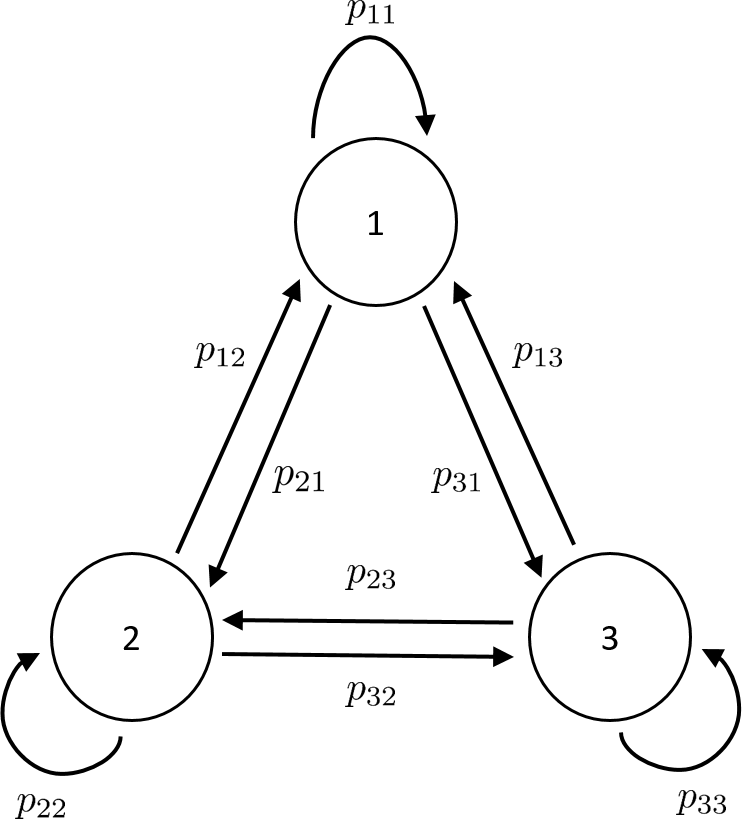
\includegraphics[width=0.6\textwidth]{network1.png}
       \caption{This is a connected network model in 3 dimensions. Each patch is connected with both its neighbors and itself, with edge weights denoted by $p_{ij}$ which represent the proportion of population transferred from patch $j$ to $i$ in a single year. \label{fig1}}
\end{center}
\end{figure}

The population of each node at each time $t$ is stored in the state vector $\mathbf{s}_{t}$, an $n$ dimensional column vector defined as
\begin{equation}\label{statevector}
\mathbf{s}_{t} = 
\begin{bmatrix}
s_{t,1} \\
\vdots \\ 
s_{t,i} \\
\vdots \\ 
s_{t,n}
\end{bmatrix},
\end{equation}
where element $s_{t,i}$ represents the number of individuals in node $i$ in year $t$. We define a mapping of state vector $\mathbf{s}_{t}$ from year $t$ to $t+1$ as
\begin{equation}\label{generalmodeleq}
\mathbf{s}_{{t+1}} = \textbf{P}\textbf{g}(\mathbf{s}_{t}),
\end{equation}
with the vector function 
\begin{equation}\label{vectorlogmap}
\textbf{g}(\mathbf{s}_{t}) = 
\begin{bmatrix}
g(s_{t,1}) \\
\vdots \\ 
g(s_{t,i}) \\
\vdots \\ 
g(s_{t,n})
\end{bmatrix}.
\end{equation}

Thus by applying the growth function defined in Equation \ref{logisticmap} element-wise to each patch in $\mathbf{s}_{t}$ and multiplying the transition matrix $\bf{P}$ by the resulting column vector $\textbf{g}(\mathbf{s}_{t})$, we have our $n$ dimensional determinstic network model of population growth and spread on the network.

\section{Analysis of 2-Dimensional System}

With the new notation in mind, we can describe the most general case of a two-patch system for analysis:
\begin{equation}\label{2d.1}
s_{t+1,1} = f_1(\mathbf{s}_{t}) = \frac{p_{11}s_{t,1}e^r}{1+\frac{s_{t,1}(e^r-1)}{K}} +
\frac{p_{12}s_{t,2}e^r}{1+\frac{s_{t,2}(e^r-1)}{K}}
\end{equation}
\begin{equation}\label{2d.2}
s_{t+1,2} = f_2(\mathbf{s}_{t}) = \frac{p_{22}s_{t,2}e^r}{1+\frac{s_{t,2}(e^r-1)}{K}} +
\frac{p_{21}s_{t,1}e^r}{1+\frac{s_{t,1}(e^r-1)}{K}}.
\end{equation}
Similarly to the 1-dimensional analysis, we want to find the fixed points of the above system, $s_1^*$ and $s_2^*$. We define $s_i^*$ as the fixed point value of patch $i$ in the state vector, where $f_i(s_i^*) = s_i^*$. Checking for the fixed points as we did before, we find that the extinct state at $(0,0)$ remains. Intuitively following the results from the 1-dimensional analysis, we predict the existence of a stable positive non-zero state. If we assume symmetry in our transition matrix, meaning in this case that $p_{12} = p_{21}$, because column sums also equal $1$, we find that $p_{11} + p_{12} = 1$ and $p_{21} + p_{22} = 1$. Simplifying the system with this assumption, we find the fixed point to be $(K, K)$, as predicted. Without this assumption of symmetry, in the model's most general form, we must solve a complicated polynomial equation to arrive at an analytical form for the positive fixed point. We do not attempt to solve it here.

\subsection{Stability Analysis}

As in the 1-d analysis, we investigate the stability of the extinct state. From Strogatz (1994), we can characterize the stability of this fixed point from the Jacobian matrix $J$, below, which describes our system of equations:
\[
J = 
\begin{bmatrix} 
\frac{\partial f_1}{\partial s_1} & \frac{\partial f_1}{\partial s_2} \\
\frac{\partial f_2}{\partial s_1} & \frac{\partial f_2}{\partial s_2}
\end{bmatrix}.
\]
We can characterize the stability of the extinct state by determining the eigenvalues of the Jacobian evaluated at that point. We evaluate the Jacobian at $(s_1^*,s_2^*) = (0,0)$ below:
\[
J_{0,0} = 
\begin{bmatrix} 
p_{11}e^r & p_{12}e^r \\
p_{21}e^r & p_{22}e^r
\end{bmatrix}
\].
We allow the carrying capacity $K$ to be equal to one. As a result, the population terms are taken to represent a fraction of the total carrying capacity.
\\

Setting up the characteristic equation for the Jacobian,
$$(p_{11}e^r - \lambda)(p_{22}e^r - \lambda) - p_{21}e^rp_{12}e^r = 0,$$
we solve for the eigenvalues using the quadratic equation,
\begin{equation}\label{roots}
\lambda_+, \lambda_- = \frac{e^r\left(p_{11} + p_{22} \pm \sqrt{(p_{11}-p_{22})^2 + 4p_{21}p_{12}}\right)}{2},
\end{equation}
where $\lambda_+$ denotes the root derived from adding the quantity under the square root, and $\lambda_-$ denotes the result of subtracting it. We note that in our model, movement between nodes conserves population such that the column sums of the transition matrix $\textbf{P}$ are equal to 1. Thus, $p_{11} = 1-p_{21}$ and $p_{22} = 1- p_{12}$. Substituting these into Equation \ref{roots}, we get:
\begin{equation}\label{2dstabilityconserve}
\lambda_+, \lambda_- = \frac{e^r\left[p_{11} + p_{22} \pm (2-p_{11}-p_{22})\right]}{2}.
\end{equation}
We can simplify this to get an expression for each eigenvalue: 
$$\lambda_+ = e^r$$
$$\lambda_- = e^r(p_{11}+p_{22} - 1).$$
Recall that the elements of $\textbf{P}$ represent the proportion of population transferred between nodes. As such, they are bounded between $0$ and $1$. Because $0 \leq p_{11} \leq 1$ and $0 \leq p_{22} \leq 1$, it follows that $-1 \leq p_{11} + p_{22} - 1 \leq 1$. Thus the magnitude of $\lambda_-$ will always be a fraction of $\lambda_+$, such that $|\lambda_-| \leq |\lambda_+|$. To determine stability, we need only look at the magnitude of the larger eigenvalue, $\lambda_+$. If the magnitude of $\lambda_+$ is less than 1, then the fixed point is stable, and conversely if the magnitude of $\lambda_+$ is greater than 1, the fixed point is unstable. Setting up the inequality $\lambda_+ > 1$, we find that for $r > 0$, the fixed point at $(0,0)$ is unstable. We have then shown that in 2-D, the extinct state is unstable when the growth rate $r$ is positive.

\section{Numerical Methods}
Due to the complexity of analyzing the general network model in higher dimensions, in this section we introduce the deterministic models we use for numerical simulations. This includes the discrete map as well as an integrated ODE model. 

\subsection{Discrete Map}
The discrete map defined by Equation \ref{generalmodeleq} was implemented in R directly and was used for all results in the small world network section in Chapter 3.

\subsection{ODE Model}
We used an integrated ODE model to compare against the stochastic model in the stochastic modeling section. To see whether our discrete map derivation agrees with the original ODE model, we generate an integrated ODE model using the 'deSolve' package with the logistic equation (\ref{logisticode}) which we modify to incorporate the immigration and emigration terms derived from the transition matrix $\textbf{P}$ in Equation \ref{transtionmatrix}. We define this as:
\begin{equation}\label{odecompmodel}
\frac{dN_i}{dt} = rN_i\left(1-\frac{N_i}{K}\right) + \sum_{j = 1, j \neq i}^{n}p_{ij}N_j - \sum_{j=1,j \neq i}^{n}p_{ji}N_i.
\end{equation}
The term $p_{ij}N_j$ is the number of individuals patch $j$ sends to patch $i$. The immigration term then, is the sum of $p_{ij}N_j$ over all patches $j$ that are not the patch in question, $i$. Emigration is defined similarly, though it is the sum of all outgoing individuals, $p_{ji}N_i$ over all patches that are not the original patch $i$. 

The values of $p_{ij}$ in the transition matrix are filled using the migration rate $v$, which is a newly introduced parameter specified prior to beginning a simulation. In our simulations, we assume that edges between nodes are equally weighted with value $v$. Recall element $p_{ij}$ is the proportion of population each patch transfers out over a yearly time step. For every edge $p_{ij}$ where there exists a connection, we set its weight to $v$. Because the population is conserved, the values along the matrix diagonal values are set by the equation: $$p_{jj} = 1 - k_jv,$$ where $k_j$ is the out degree of patch $j$. An example of a network generated with migration rate $v$ is shown in Figure \ref{networkv}.

\begin{figure}[t!]
\begin{center}
       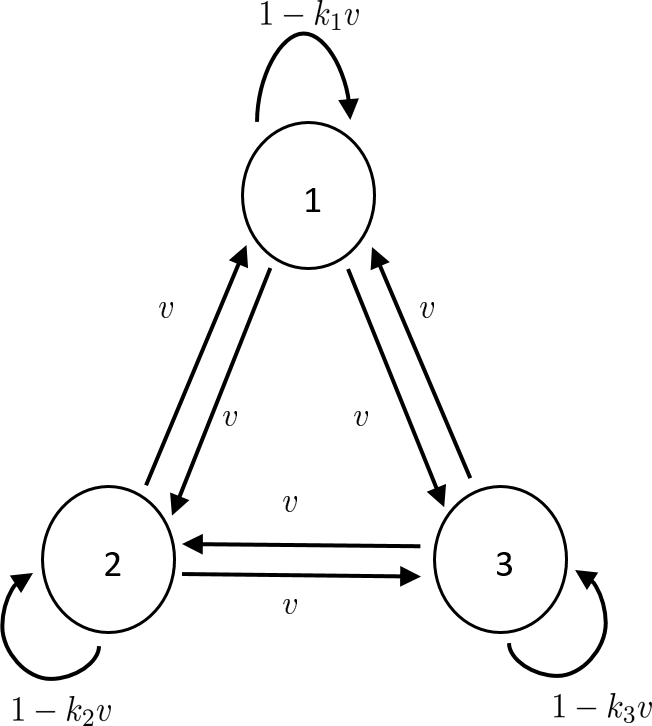
\includegraphics[width=0.5\textwidth]{networkv.png}
       \caption{Figure showing a sample network with edges equally weighted. The parameter $v$ is the migration rate between nodes and $k_j$ is the out degree of the node $j$. In this example $k_j = 2$ for each node. \label{networkv}}
\end{center}
\end{figure}

To simulate a biotic invasion over a given time period, we initialize the state vector as $\mathbf{s}_{0} = \vec{0}$. Then, we set the value of the patch where the invasion begins to carrying capacity $K$. Then we apply the particular model, discrete map, integrated ODE, or Monte Carlo, which will be introduced later, for the given time period. We discuss the agreement of the deterministic models, the discrete map and the integrated ODE, in the following section. 

\subsection{Deterministic Model Agreement}

The discrete map model in Equation \ref{generalmodeleq} differs from the ODE model presented in Equation \ref{odecompmodel} in how population is distributed. In the former discrete time model, population is grown according to the growth function, Equation \ref{vectorlogmap}, before migration is calculated at the end of each time step according to the transition matrix. In the continuous time integrated ODE model, population growth and migration are calculated concurrently. This creates a small discrepancy between the models, which can be assumed to be negligible for our purposes. Consider the equation $\frac{dN_i}{dt} = -vN_i$, which represents the population loss term due to outbound migration on node $i$. Integrating over the course of one year gives us the equation $N_i(t+1) = e^{-v}N_i(t)$. The corresponding system in our discrete map model is $N_i(t+1) = (1-v)N_i(t)$. At low values of $v$, $e^{-v} \approx 1-v$. In this thesis, we typically use values of $v << 1$ as well as $r << 1$. We show the agreement of the model for typical parameter values in Figure \ref{odemap1}. Disagreement at a large value for $v$ is shown in Figure \ref{odemap2}. To find the exact parameter relationships in higher dimensions we would have to integrate the differential equation represented in \ref{odecompmodel}, but are unable to do so. Despite this, we observe that at the typically parameter values chosen in this study, there is agreement between the two deterministic models presented.

\begin{figure}[t!]
\begin{center}
       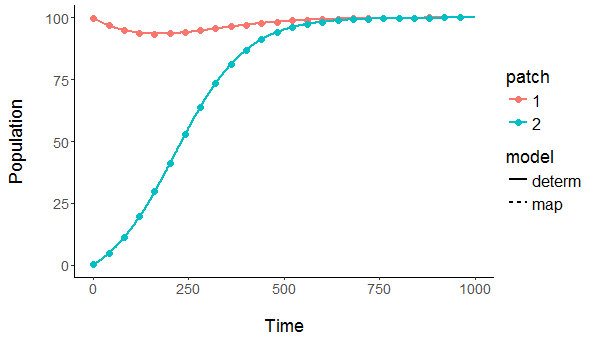
\includegraphics[width=1.0\textwidth]{odemap1.png}
       \caption{Figure showing the agreement between the ODE model and the discrete map at typical parameter values. The solid lines are the abundances in the ODE model, and are overlaid with points every $40$ years from the discrete map model. The parameter values given are listed: $n = 2$ patches, migration rate $v = 0.001$, birth rate $r = 0.01$, and carrying capacity $K = 100$, over a course of $1000$ time steps. \label{odemap1}}
\end{center}
\end{figure}
\begin{figure}[t!]
\begin{center}
       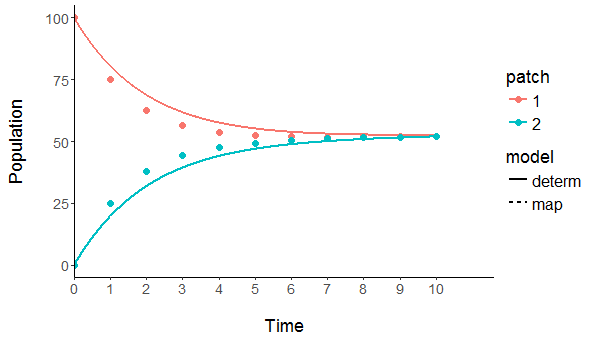
\includegraphics[width=1.0\textwidth]{odemap2.png}
       \caption{Figure showing discrepancy between the ODE model and the discrete map at a large $v$ value. The points are plotted at every $1$ year. The parameter values given are listed: $n = 2$ patches, migration rate $v = 0.25$, birth rate $r = 0.01$, and carrying capacity $K = 100$, over a course of $10$ time steps. \label{odemap2}}
\end{center}
\end{figure}

\chapter{Small World Networks}
\section{Background}
Networks are often characterized by commonly studied properties of their nodes and edges. Two of these properties are called the clustering coefficient and characteristic path length. As discussed in \cite{watts1998collective}, the clustering coefficient depends on triplets of nodes. Consider a vertex $V$ with $k_V$ neighbors on an undirected graph. Any connection between the neighbors of $V$ generates a node triplet. Then there can exist at most $k_V(k_V-1)/2$ edges between the $k_V$ neighbors. Let clustering coefficient $C_V$ denote the fraction of these triplets that actually exist for node $V$. Then, the average clustering coefficient $C$ is the average of $C_V$ calculated from each vertex. The characteristic path length, $L$ of a graph is the shortest path length between two vertices, averaged over all unique pairs of vertices. 

Regular networks are defined as networks where each node has the same number of neighbors, and the connections between neighbors follow a particular pattern. An example of a particular pattern on a ring is shown in Figure \ref{smallworld}. Random networks are defined wherein the connections between nodes are determined randomly. It is a common property of regular networks to be highly clustered. Random networks, on the other hand, exhibit lower clustering but have small characteristic path lengths due to the existence of many randomly introduced connections between distant nodes \citep{walsh1999search}. Small world networks were introduced by \cite{watts1998collective} as being an intermediate between these two types of networks. They maintain some degree of regularity in node connections while also having a small number of random connections relative to a completely random graph.

We are interested in small world networks because they could be analogous to the movement network of invasive species. Population networks of invasive species often develop by a combination of movement between neighboring habitats and dispersal along a long distance transport vector, for example, a truck carrying a soil shipment across the United States. Indeed, there have been many research papers discussing small-world properties of real world networks, including transportation networks \citep{latora2001efficient}. By analyzing the impact of randomness on a small world network, we hope to learn about the effect of long-distance dispersal in biotic invasions.

\section{Small World Methods}

The original paper \citep{watts1998collective} generates a small world network by rewiring a regular ring lattice into a random graph. We begin with the regular ring lattice, which we define as a regular network where the nodes are arranged into a ring, and begin randomly choosing edges and randomly reassigning their endpoints, based on a parameter of rewiring probability $p$. An example of this process is shown in Figure \ref{smallworld}. 

\begin{figure}[t!]
\begin{center}
       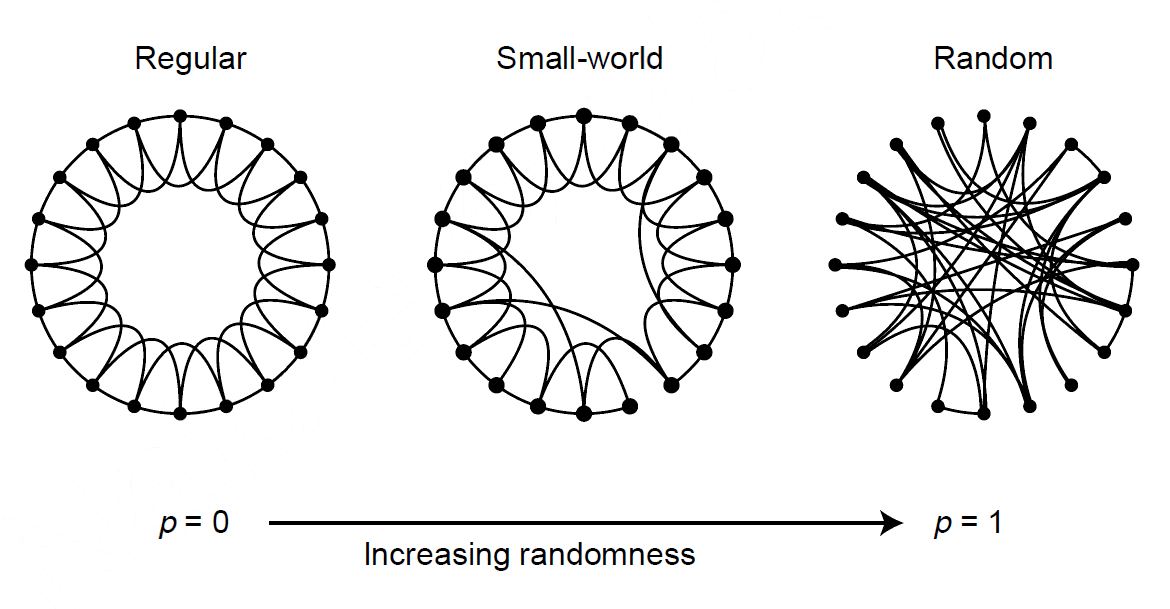
\includegraphics[width=0.9\textwidth]{smallworld.png}
       \caption{A regular ring lattice is rewired with increasing values of $p$, the rewiring probability. \label{smallworld}}
\end{center}
\end{figure}  

The increase in rewiring probability is correlated with a decline in characteristic path length and mean clustering coefficient, seen in Figure \ref{pathlength_igraph}.

\begin{figure}[t!]
\begin{center}
       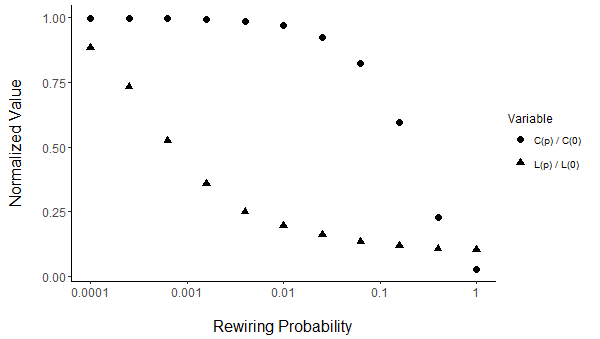
\includegraphics[width=0.9\textwidth]{paths.png}
       \caption{Plots showing relationship between normalized characteristic path length and clustering coefficient with rewiring probability. $C(p)$ and $L(p)$ refer to the values of each property for a network generated with given rewiring probability $p$. The plotted values are normalized by their values calculated on a regular graph. Parameter values are $n = 1000$, $m = 5$, the results are averaged over $20$ realizations.\label{pathlength_igraph}}
\end{center}
\end{figure}  

\subsection{Extension to Invasion Model}

In this section we implement a portion of the procedures including generating the small world network in R using the package `igraph' \citep{csardi2006igraph}.

The algorithm for constructing the small world network using igraph begins by constructing a ring lattice with each of the $n$ nodes connected to its nearest $2m$ neighbors. We choose $m = 2$ and $n = 50$. Begin the rewiring process by choosing nodes $x$ and $y$ from a random uniform probability distribution of all possible node values. Rewiring is done by replacing each edge $e_{ij}$ with edge $e_{xy}$ with probability $p$. Rewiring events resulting in a self-loop or a duplicated path are redrawn by the igraph algorithm, by redrawing another pair of values $x$ and $y$. We imposed an additional check at the end of the rewiring process so that any disconnected networks, meaning networks where there are unreachable nodes, were entirely discarded and replacement networks were generated. This implementation slightly differs from the original Watts and Strogatz method in that both endpoints of the edge $e_{ij}$ are randomized here as opposed to just one in the original method. However, this difference did not seem significant to the underlying small world network properties. To validate the igraph method we created a plot of characteristic path length and clustering coefficient in Figure \ref{pathlength_igraph} and compared the results with those presented in \cite{watts1998collective}. We found that the curves were almost identical, with an insignificant difference attributed to an algorithmic difference between the `igraph' small world network generation and the algorithm presented in the original paper.

To adapt this small world network to fit our model of species invasion, we transform its adjacency matrix. The adjacency matrix of a network is defined as a matrix $\textbf{A}$ such that every element $a_{ij}$ has a binary value $1$ or $0$. A value of $1$ indicates a connection between nodes $i$ and $j$ whereas $0$ indicates no connection. Because the small world network is undirected, the adjacency matrix is symmetric, so that $a_{ij} = a_{ji}$. 

To map the adjacency matrix to the transition matrix, we perform the following transformations:
\begin{center}
\begin{enumerate}
\item $p_{ij} = va_{ij}$ for $i \neq j$\\
\item $p_{jj} = 1 - \sum_{i = 1}^{n}va_{ij}$.
\end{enumerate}
\end{center}
In this definition, $\textbf{P}$ refers to the transition matrix defined in Equation \ref{transtionmatrix}, and $v$ is the migration rate, the proportion of population sent from any node to every other node.

Consider the network in Figure \ref{sample_smallworld} of $50$ nodes labeled from $1$ to $50$ counterclockwise in a ring lattice. We use the transformed adjacency network to map an invasion with yearly time steps over the course of 1000 years. We investigate the transient properties of this system by recording a metric $t(p)$, called the time to establishment. We define this metric on a network rewired with probability $p$, as the number of time steps it takes for the population to spread from the initial node $1$ to the one diametrically opposite, node $26$, and surpass a population threshold arbitrarily set to $100$ individuals.

Consider one experiment to be defined as generating a small world network with rewiring probability $p$, transforming the adjacency matrix, and running a simulation as described above.

We performed several sets of experiments recording $t(p)$ at different values of $p$ and averaged the results over $1000$ networks for each value of $p$, with the average times to establishment denoted by $T(p)$. In each set of experiments, we varied values of $v$ and $r$ to observe the effects of migration rate and birth rate on the transient properties of an invasion on our network model. The results are presented in the next section.

\begin{figure}[t!]
\begin{center}
       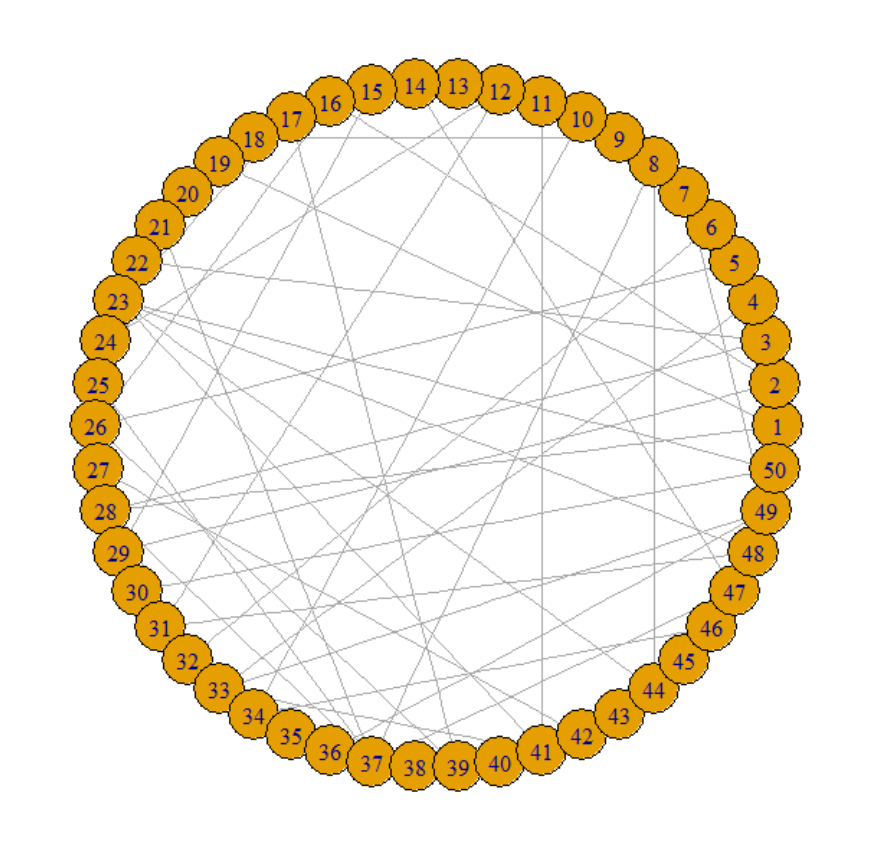
\includegraphics[width=0.7\textwidth]{sample_smallworld.png}
       \caption{Example of the small world network generated by igraph with $n = 50$, $m = 2$, and $p = 0.25$.\label{sample_smallworld}}
\end{center}
\end{figure}  

\section{Results}

We first present the results of normalized time to establishment, that is, $T(p)/T(0)$, versus the rewiring probability $p$, with varying migration rates $v$ in Figure \ref{smallworld_v}. We next present the results of varying the birth rate $r$ in Figure \ref{smallworld_b}. Then, we present results where $v$ and $r$ are varied respectively to each other. The migration and birth rate terms are both linear order in population $N$, so varying both at the same time in opposing directions attempts to show the relative effects of each parameter while keeping the overall time scale of the invasion reasonably constant. The results of the normalized time to establishment for this set of experiments is shown in Figure \ref{smallworld_allnorm}, and the non-normalized, absolute time results are presented in Figure \ref{smallworld_allabs}. 

\begin{figure}[t!]
\begin{center}
       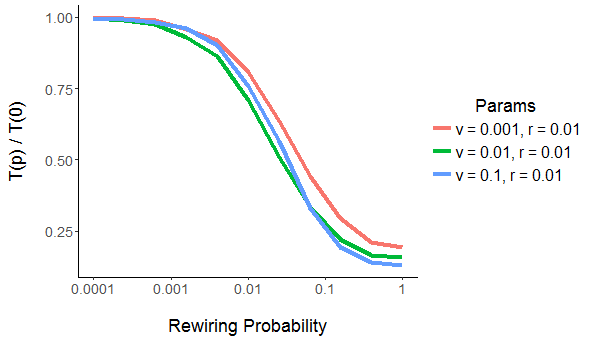
\includegraphics[width=0.8\textwidth]{smallworldvaryv_norm.png}
       \caption{Plot of the normalized time in years to establishment of a species invading a small world network with varying values of $v$. Parameters $n = 50$, $m = 2$, $r = 0.01$, $K = 5000$, and establishment threshold is set at $100$. Rewiring probability is parameter $p$.\label{smallworld_v}}
\end{center}
\end{figure}
\begin{figure}[t!]
\begin{center}
       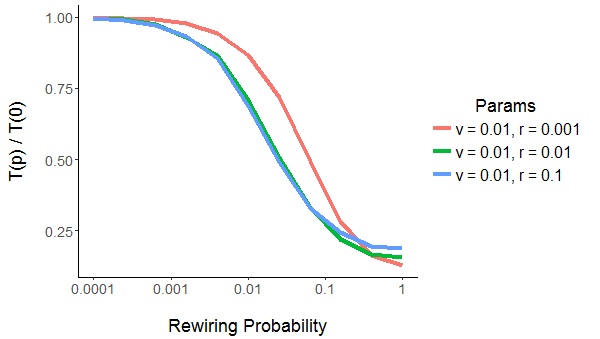
\includegraphics[width=0.8\textwidth]{smallworldvaryb_norm.png}
       \caption{Plot of the normalized time in years to establishment of a species invading a small world network with varying values of $r$. Parameters $n = 50$, $m = 2$, $v = 0.01$, $K = 5000$, and establishment threshold is set at $100$. Rewiring probability is parameter $p$.\label{smallworld_b}}
\end{center}
\end{figure}
\begin{figure}[t!]
\begin{center}
       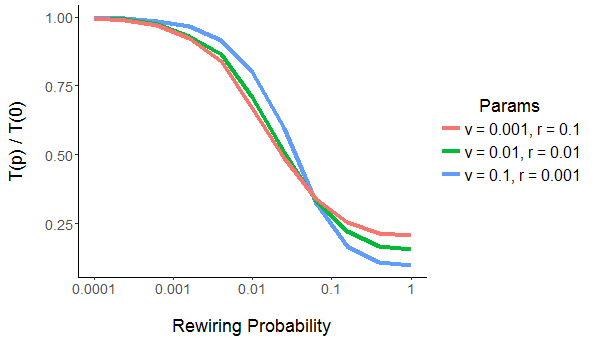
\includegraphics[width=0.8\textwidth]{smallworld_allnorm2.png}
       \caption{Plot of the normalized time in years to establishment of a species invading a small world network with varying sets of migration rates $v$ and birth rate $r$. Parameters $n = 50$, $m = 2$, $r = 0.01$, $K = 5000$, and establishment threshold is set at $100$. Rewiring probability is parameter $p$.\label{smallworld_allnorm}}
\end{center}
\end{figure}  

\begin{figure}[t!]
\begin{center}
       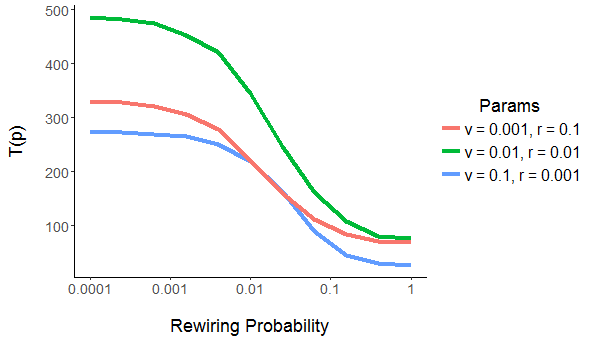
\includegraphics[width=0.8\textwidth]{smallworld_allabs2.png}
       \caption{Plot of the absolute time in years to establishment of a species invading a small world network with varying sets of migration rates $v$ and birth rate $r$. Parameters $n = 50$, $m = 2$, $r = 0.01$, $K = 5000$, and establishment threshold is set at $100$. Rewiring probability is parameter $p$.\label{smallworld_allabs}}
\end{center}
\end{figure}  

Comparing the plots of normalized time to establishment to Figure \ref{pathlength_igraph}, we find that the normalized time to establishment, $T(p)/T(0)$, shares the same shape as $C(p)/C(0)$. This is interesting because we expected these curves to relate to the characteristic path length since the characteristic path length is directly related to the number of long-distance connections between distant nodes on the ring. It is not immediately clear why the time to establishment should appear more analogous to the clustering coefficient than the characteristic path length, but this warrants further investigation.

Following the curves in the Figure \ref{smallworld_v}, we find that starting from $p = 0$, the curves diverge and settle at $p = 1$ such that the larger $v$ is, the smaller $T(1)/T(0)$ is at $p = 1$; they are inversely related. This result is as expected as we hypothesized a relationship between decreased characteristic path length and increasing speed of invasion (time to establishment). This is reasonable, as in a highly connected graph with high migration rate, the first few time steps could find the invasive species spread all around the network, whereas this would not occur as quickly with a slower migration rate.

Following the curves in the Figure \ref{smallworld_b}, we find a surprising result. First, we notice that whereas previously observed curves were fairly close together, at very low birth rate, the time to establishment drops off at a higher value of $p$ than at higher birth rates. Secondly, we notice that the normalized time to establishment at $p = 1$ is directly related to the birth rate. Note that we are plotting the normalized time to establishment. The absolute time to establishment is positively related to increasing values of both $v$ and $r$. The fact that the normalized time to establishment at $p = 1$ is inversely related to birth rate, such that the curve with the lowest growth rate exhibits the lowest normalized time to establishment at $p = 1$ can be explained by considering the contribution of long distance connections in the spread of the invasion. One possible explanation is that the long distance connections contribute more in invasions with low birth rate because the time it takes for an invasion to spread via diffusion across the network would be much longer than for an invasion with a higher growth rate. Thus, at low values of $p$, the invasion process is extremely slow with low birth rate, but increases rapidly with an increasing number of long distance connections. This could also explain the large gap between the curves. Perhaps this phenomenon is only visible at sufficiently low birth rate. 

By varying both parameters $v$ and $r$ concurrently, in Figure \ref{smallworld_allnorm}, we see that values of the time to establishment at $p = 1$ supports the results from varying the parameters separately. However, if we look at the absolute time plot in Figure \ref{smallworld_allabs}, we notice two main differences. Note the change on the y-axis to the number of years, rather than a normalized value. First, we notice that while the values of $T(p)/T(0)$ between the curves diverge as $p$ increases, the absolute time values of $T(p)$ converge as $p$ increases. One possible reason for this is that in the initial regular graph, the shortest path between opposite nodes is longer than in the random graph. Different combinations of parameters $v$ and $r$ could produce slower or faster spreading invasions. As that path length decreases as $p$ increases, any difference in the spread rate between parameter combinations is diminished since there is less distance to cover. 

Additionally, we find that the curves tracing absolute time to establishment vs. $p$ converge in a different order at $p = 1$ than those of normalized time to establishment. Here, the curve with the intermediate value of $v$ and the lowest value have switched places. It seems that in absolute terms, the curve with $v = 0.1$ still results in the fastest establishment. There is possibly some interplay between these parameter values and invasion dynamics that we do not completely understand.

\chapter{Stochastic Modeling}

\section{Stochastic Model}
The stochastic simulations are carried out in a continuous-time Monte Carlo simulation using the Gillespie algorithm \citep{gillespie1977exact}. Generally, we calculate what happens over a series of time steps, where in each time step one individual is either born, dies, or migrates between nodes. We keep track of the number of individuals in each patch and determine what happens at each time step based on the probability of each state transition: birth, death, or migration. 

The birth and death rates $b_i$ and $d_i$ respectively, for a population $N_i$ in each node, were chosen as:
\begin{equation}\label{birth}
b_i = rN_i
\end{equation}
\begin{equation}\label{death}
d_i = r\frac{N_i^2}{K}.
\end{equation}
This choice is easily related back to the logistic ODE in Equation \ref{logisticode}. We can expand the equation and rearrange the terms as:
\begin{equation}\label{bdode}
\frac{dN}{dt} = rN - r\frac{N^2}{K},
\end{equation}
where the birth and death rates are represented by the positive and negative terms respectively.

The total migration rate $M$ is defined as the total number of individuals in the state vector. This is because each individual has a possibility of migrating. However, the majority of migrations are self-loops, which do not result in any population transfer. Notice this migration rate is defined as the total migration rate for the implementation of the Monte Carlo simulation, and is different from $v$, the parameter which relates to individuals that actually migrate out of a node:
\begin{equation}\label{stochmigrationrate}
M = \sum_{i = 1}^{n}N_i.
\end{equation}

Transitioning between different population states is a Poisson process with a mean rate of $R_{tot}$. $R_{tot}$ is equal to the sum of all birth, death, and migration rates,
$$R_{tot} = \sum_{i}^{n}b_i + \sum_{i}^{n}d_i + \sum_{i}^{n}N_i,$$ 
and the time between events is then exponentially distributed with mean $R_{tot}^{-1}$. 

The algorithm to simulate a biotic invasion is implemented as described:
First, initialize the state vector $s_t$ as described for the deterministic models.
At each time step, record the values in each patch in $s_t$.
To generate the time to the next event $\tau$, we first draw a uniformly distributed random number $u \in (0,1]$. This is converted to an exponentially distributed number by:
\begin{equation}\label{uniftoexp}
\tau = \frac{\ln(\frac{1}{u})}{R_{tot}}.
\end{equation}
After we have found the time step, we determine whether a birth, death, or migration event has occurred. This is done by assigning a numerical range to each event proportional to the fraction of its rate over the total rate $R_{tot}$, then seeing where $u$ falls relative to these ranges after normalizing it to the total rate. Specifically, we first multiply $u$ by the total rate $R_{tot}$. Then, we decide which type of event occurs. If the relation $R_tot < M$ is true, a migration event occurs. Otherwise, we know a birth or death event has occurred. To decide between the two, we generate another random uniform number $u$, and multiply it by the sum of the birth and death rates. Then we perform the test $\sum_{i}^{n}b_i + \sum_{i}^{n}d_i < \sum_{i}^{n}b_i$. If the result is true, then a birth occurs, and otherwise, a death occurs. 

We repeat the process of drawing uniform random numbers and placing them within a range to determine which patch or patches are involved in the event that occurs. For birth and death this involves drawing $u$, then multiplying by the total number of individuals in the state vector. To determine which patch the birth occurs in, we follow a similar process as described in the previous paragraph in assigning each patch a birth rate as defined in Equation \ref{birth} and testing whether the process occurs in each path consecutively, stopping if we find the one where birth occurs. Death is determined in a similar manner using the equation \ref{death}. 

For migration the process involves drawing two numbers, one for the source node and one for the destination node. To determine the source node, we first multiply the number $u$ by the total number of individuals in the state vector. The process of determining which patch is the source is the same as above, but the rate value we assign to each patch is simply the number of individuals in that patch. To determine the destination node, the rate is determined by the value of $p_{ij}$ from the transition matrix, where $j$ would be the source node we just found and we iterate through values of $i$ to find the destination.

To generate a plot of population vs. time that we can compare against the deterministic model, we run the algorithm described above for $1000$ years.

\subsection{Results}
In the introduction we stated that a large proportion of invasive species introductions do not establish stable colonies, and that those that do experience a lag period before growing. However, in the deterministic model analysis section, we showed that the extinct state of our population growth function is unstable. This means deterministically we would expect any introduction to grow to carrying capacity. The difference between the deterministic model and biological reality is that in reality stochastic effects can play a large role in a colony's establishment. Stochastic effects are particularly significant in populations with a small number of individuals and small migration rates, both of which are properties of invasive species introductions. 

Here we present some results from the comparison of the deterministic ODE model and the stochastic Monte Carlo simulation. The following are multi-panel plots of 1000-year simulations of the deterministic model (solid line) and the stochastic model (dashed line) with constant parameter values $K = 500$, $r = 0.01$. We initialize the invasion in patch $1$ and record its spread to patches $2$ and $3$. These figures illustrate the increasing magnitude of stochastic effects at low population levels and migration rates.

\begin{figure}[t!]
\begin{center}
       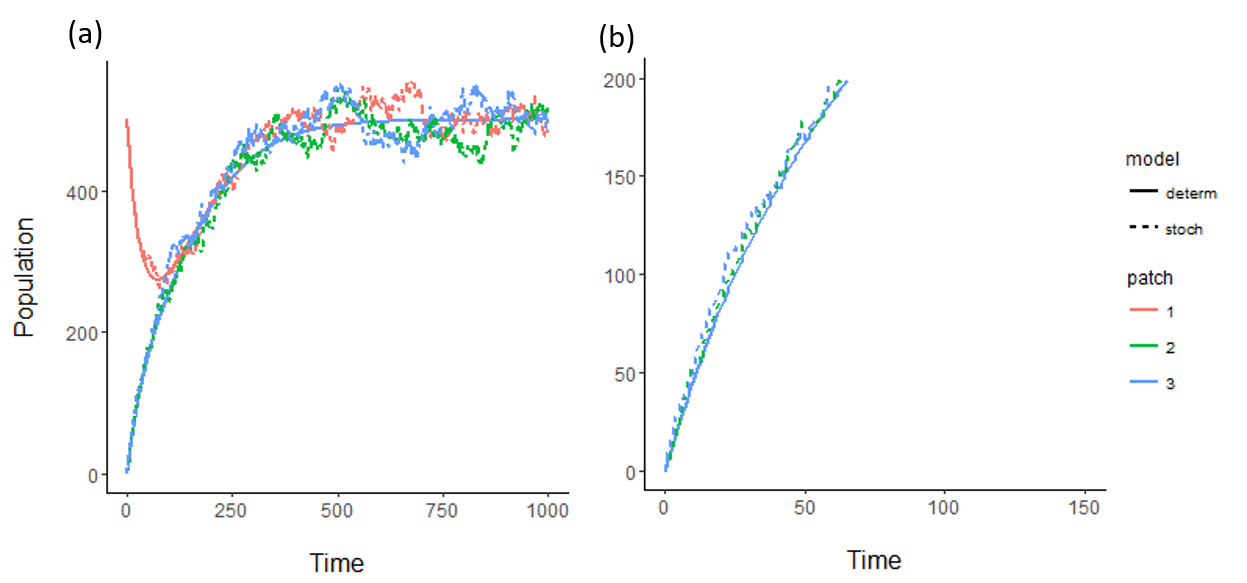
\includegraphics[width=1.0\textwidth]{combinedv01.png}
       \caption{Migration rate $v = 0.01$. Plot (a) shows the entire 1000-year trajectory of each population patch while plot (b) shows a shorter time frame where stochastic effects are most apparent. Other parameters $K = 500$, $r = 0.01$.\label{combinedv01}}
\end{center}
\end{figure}  

\begin{figure}[t!]
\begin{center}
       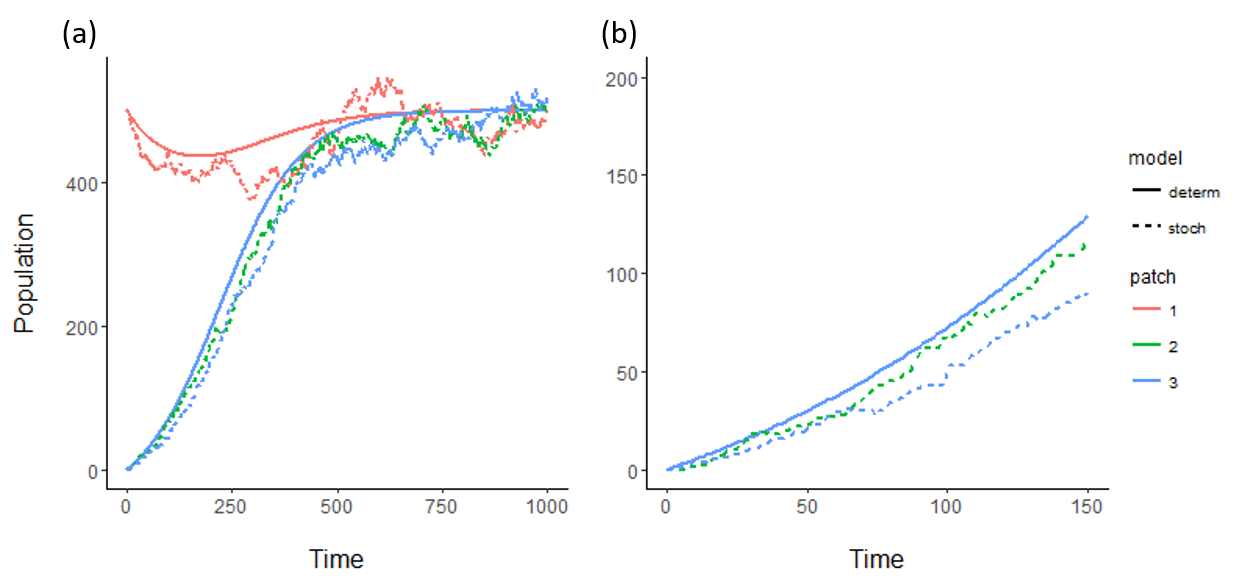
\includegraphics[width=1.0\textwidth]{combinedv001.png}
       \caption{Migration rate $v = 0.001$, other parameters $K = 500$, $r = 0.01$.\label{combinedv001}}
\end{center}
\end{figure}  

\begin{figure}[t!]
\begin{center}
       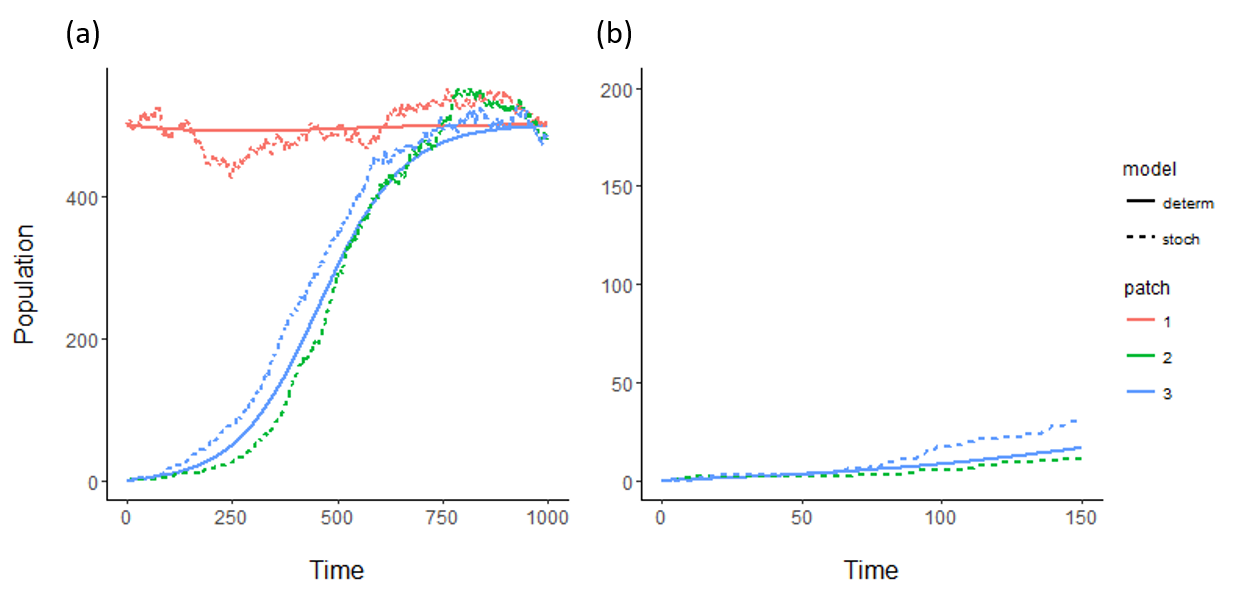
\includegraphics[width=1.0\textwidth]{combinedv0001.png}
       \caption{Migration rate $v = 0.0001$, other parameters $K = 500$, $r = 0.01$.\label{combinedv0001}}
\end{center}
\end{figure}  

\begin{figure}[t!]
\begin{center}
       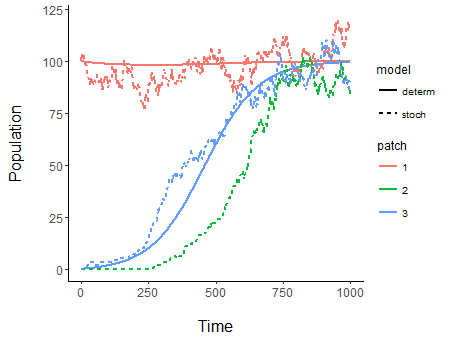
\includegraphics[width=0.8\textwidth]{pop100stochv0001.png}
       \caption{Migration rate $v = 0.0001$, other parameters $K = 100$, $r = 0.01$. This plot shows that patch dynamics can become highly varied when the population sizes are low. \label{pop100stochv0001}}
\end{center}
\end{figure}  
We note that in all of these simulations, the overall pattern is that all populations reach equilibrium. This is reasonable because our birth and death processes mimic the logistic growth function, which has an unstable extinct state. At low population, the migration out of a patch is negligible, so the probability of a series of chance events driving a new population experiencing logistic growth to extinction is incredibly small when there is a source feeding into it. As a result the stochastic model more or less traces the deterministic model with small perturbations.

However, these figures show that the fit between the deterministic and stochastic model breaks down over certain time and parameter regimes. Specifically the regime where stochastic effects are most apparent is in the initial lag period before logistic growth is high, when population is low and population dynamics are primarily controlled by migration. While in the deterministic model, the populations in patches $2$ and $3$ grow at the same rate, this is not true of the stochastic model. Due to low migration rates and birth rates at low population, if one of the sink patches happens to receive an introduction early on, its population will grow much more rapidly than the others, as seen in Figure \ref{pop100stochv0001}. 

Previously we discussed Allee effects as more biologically realistic than logistic growth models. The subject of Allee effects in stochastic simulations is discussed in the concluding chapter as a possible topic of future work.

\chapter{Conclusions}
\section{Summary}
In this section we will summarize the results of this thesis. We first developed our $n$ dimensional deterministic network model and analyzed it. We found the fixed points and stability of the $1$ dimensional system, which is simply logistic growth of a single population, to be the same for our discrete map in Equation \ref{logisticmap} as the stability of the original continuous logistic equation (\ref{logisticode}) from which it was derived. For populations with a positive growth rate $r$, we find that the extinct state is unstable while there is a stable fixed point at the carrying capacity $K$. We presented a portion of the analysis of the $2$ dimensional system, though did not include calculations for a positive non-zero fixed point due to its complexity. We found that the stability result for the extinct state held in the more complex $2$ dimensional system. This result was that the extinct state is unstable. For modeling higher dimensional networks, we relied on numerical simulations.

We implemented deterministic and stochastic versions of this model in R. We explained how the discrete time map we developed in Equation \ref{logisticmap} differs from the integrated ODE model in Equation \ref{odecompmodel} in dependence on parameters $v$ and possibly $r$. We found that the discrepancy is negligible for relevant parameter values in this study and leave it for future work to determine the exact relationship between the discrete time and continuous time models.

We introduced small world networks and used them to study the effects of random dispersal events on the transient properties of a biotic invasion. We measured the speed of an invasion by measuring a metric called time to establishment. This was the time it took for an invasive population establish on the diametrically opposite node from where the invasion began. We recorded the normalized and absolute time to establishment for multiple parameter sets at increasing values of $p$, the rewiring probability of the small world network generator. We found that the normalized time to establishment generally decreases in relation to rewiring probability, which we hypothesize relates to a decrease in characteristic path length with increasing $p$, resulting in an increasing number of long distance connections between nodes, thought to be a significant component of invasive species dispersal. Further work in this area could include investigation into characteristic path length, clustering coefficient, and other network properties and how they influence spread dynamics.

We found that the results from the numerical simulations on the stochastic model generally followed a growth pattern expected from our analysis of steady states in our deterministic network model. We identified regimes where stochastic effects were most relevant: low migration rate and small population. However, we found that long-term behavior of the deterministic and stochastic models agreed. Any node that received an introduction grew its population to the carrying capacity. Allee effects would be a good direction to take future work, recalling that the stability of the extinct state switches from unstable to stable with the introduction of a strong Allee effect.

\section{Future Work}
\subsection{Allee Effect}
We previously introduced the Allee effect as an extension of the logistic growth equation. The resulting ODE incorporating an Allee effect into logistic growth is defined in Equation \ref{alleeode}. We noted that there is a difference in steady states between this model and the original ODE in Equation \ref{logisticode}. In the Allee model, there are three fixed points: $0$, $A$ (the Allee threshold), and $K$. Recall that $0 < A < K$. The extinct state, $0$ is stable, the Allee threshold is unstable, and the carrying capacity is stable. 

The difference in steady states and stability underly a significant difference between our current stochastic model and a biologically realistic one. In real landscapes introduced populations do not necessarily tend towards carrying capacity; instead, many small populations fail to establish. This effect is described by the change in steady state stability of a logistic growth model under an Allee effect. A future direction for research would be the implementation and analysis of a growth function incorporating an Allee effect. Updating the continuous time Monte Carlo simulation using birth and death rates associated with that model would likely yield interesting results when tested under low migration rate and low population. 

\subsection{Networks}
In the small world section we noted that the normalized time to establishment metric we tested followed the same shape as the normalized mean clustering coefficient. It might be fruitful to further investigate how clustering  affects spread dynamics and also what other network properties might be important in the same respect. It is not intuitively clear why clustering coefficient would impact time to establishment and so the connection may be a coincidence or related to a confounding variable, perhaps another network property that is dependent on node clustering.

Another topic of interest in many networks is the presence of hubs. Hubs, defined non-technically, are nodes which experience a large volume of of incoming and outgoing traffic relative to other nodes. As discussed in the introduction in Chapter 1, in \cite{floerl2009importance}, once an invasive species has established in a hub, it plays a large role in the spread of that species to many secondary locations, having considerable impact on the overall spread dynamics. Hubs in network models have a direct real world significance, corresponding to regions that experience large volumes of traffic, such as population and shipping centers. For example, in \cite{kaluza2010complex}, researchers found that highly trafficked ports were on coastlines that had high numbers of marine invasive species. Hubs as hotspots for the spread of invasive species could be a promising direction for future research. This type of research could be particularly useful for environmental managers, who could employ this type of knowledge to best allocate limited resources to transport hubs where they would have the largest impact.

\section{Acknowledgements}

Thank you to my incredible advisor Dr. Leah Shaw, without whom I could never have taken this project this far. Thank you for not only for demystifying mathematical analysis and always being ready to teach me something new, but for guiding me and pushing me forward through this experience and all of its ups and downs.

\bibliographystyle{plainnat}
\bibliography{bibfile}

\end{document}
